

\begin{wrapfigure}{r}{0.7\textwidth}
    %\centering
    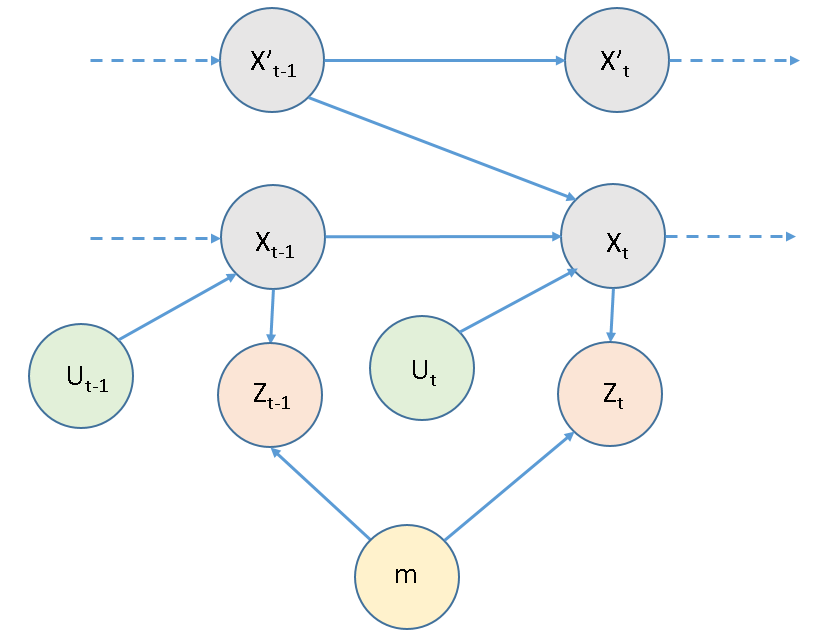
\includegraphics[width = 0.7\textwidth]{Chapters/BackgroundKnowledgeAndRelatedWork/MultiAgentTargetDetectionBackground/Figs/DBNs/Complex2TDBN.PNG}
    \caption{A DBN used for \textbf{S}imultaneous \textbf{L}ocalisation \textbf{A}nd \textbf{M}apping (SLAM), based on \cite[p.~311]{Thrun:2005:ProbabilisticRobotics}.}
    \label{fig:2TDBNExample}
\end{wrapfigure}

DBNs are a generalization of HMMs and are used to model time series. The key difference between DBNs and HMMs is that DBNs are not limited in how they decompose the hidden state variables of a complex stochastic system into the variables that represent its constituent conditional distributions \cite{AIAMA}. Rather than use a single random variable, $X_t$ to represent the state space, a set of random variables are used \cite{Murphy1994DynamicLearning}. DBNs can be considered as a special case of a Bayesian Network with an infinite number of nodes and repeating structure which specifies the transition probabilities between one time step and the next \cite[p.~204]{KollerPGM}. The hidden state variables are represented by nodes which have an associated conditional probability distribution (CPD) which states the probability of observing a value of a random variable given its parents: $p(X_i | Parents(X_i))$ \cite[p.~14]{Murphy1994DynamicLearning}. Given this representation, it is possible to calculate the joint distribution, $p(X_t | X_{t-1})$, of all $N$ state variables at time $t$ given the joint distribution at $t-1$ as \cite[p.~14]{Murphy1994DynamicLearning}:
\[
p(X_t | X_{t-1}) = \prod_{i=1}^{N}p(X_t^i | Parents(X_t^i)
\]
\citeauthor{KollerPGM} provide a technical definition of DBNs: 
"\textit{A dynamic Bayesian network (DBN) is a pair $\langle B_0, B_\rightarrow \rangle$, where $B_0$ is a Bayesian network over $X^{(0)}$, representing the initial distribution over states, and $B_\rightarrow$ is a 2-TBN for the process. For any desired time span T $\geq$ 0, the distribution over $X^{(0:T)}$ is defined as a unrolled Bayesian network, where, for any $i$ = 1, . . . , $n$:
\begin{itemize}
    \item The structure and CPDs of $X^{(0)}_i$ are the same as those for $X_i$ in $B_0$,
    \item The structure and CPD of $X^{(t)}_i$ for $t > 0$ are the same as those for $X^{'}_i$ in $B_\rightarrow$.
\end{itemize}}" \cite[p.~204]{KollerPGM}. What this essentially means is that a DBN is a compact way of specifying an infinite set of Bayesian Networks (one for each $T>0$) with repeating structure.


Technically, every DBN can be represented as a HMM and visa versa, however, the number of parameters that need to be determined to represent DBNs can be significantly less that that of HMMs \cite{KollerPGM}. For example, consider the case of $n$ discrete random variables, each with support of size $m$. Specifying the full joint distribution without assuming any conditional independences between variables would require a number of probabilities exponential in the number of random variables, $m^{n}-1$, whereas specifying the same joint distribution as factored conditional distributions may require far fewer, reaching a number of probabilities directly proportional to the number of random variables, $n \times m$ in the degenerate case \cite[p.~63]{KollerPGM}. 
%\subsubsection{A Note on Bayesian Networks}
%A Bayesian Network (BN) is a graphical way to represent a particular factorization of a joint distribution. For a detailed explanation, the reader is referred to \cite{KollerPGM}. To fully explain a complex system, it is often natural to model it as the joint distribution of a number of random variables. This is in general intractable \cite{KollerPGM}. In order to circumvent this, independence properties in the distribution can be exploited to provide a much more compact representation of the distribution. BNs exploit the fact that independence is a strong notion that doesn't often occur in the real-world; however conditional independence is a weaker property that is far more prevalent, which still leads to the desired compact representation. BNs are described by a directed acyclic graph (DAG), $G$. The nodes in the graph correspond to the random variables whose joint distribution is of interest, and the arcs represent conditional independences. Specifically, if one Burglary points to Alarm as in figure \ref{fig:BayesianNetwork}, it is implied that the distribution of Alarm is conditionally independent on all other nodes in the network given Burglary. This means that only local conditional probability distributions must be provided in order to specify the full joint distribution.

%\begin{figure}
%example bayesian network figure
%\begin{tikzpicture}[
%  node distance=1cm and 0cm,
%  mynode/.style={draw,ellipse,text width=2cm,align=center}
%]
%\node[mynode] (i) {Burglary};
%\node[mynode,below right=of i] (g) {Alarm};
%\node[mynode,above right=of g] (c) {Earthquake};
%\path %(ra) edge[latex-] (sp)
%(g) edge[latex-] (c) 
%(g) edge[latex-] (i);
%\node[left=0.45cm of i]
%{
%\begin{tabular}{cM{3}M{3}}
%\toprule
%\multicolumn{2}{c}{Burglary} \\
%\multicolumn{1}{c}{T} & \multicolumn{1}{c}{F} \\
%\cmidrule(r){1-2}
%0.001 & 0.999 \\
%\bottomrule
%\end{tabular}
%};
%\node[right=0.45cm of c]
%{
%\begin{tabular}{cM{3}M{3}}
%\toprule
%\multicolumn{2}{c}{Earthquake} \\
%\multicolumn{1}{c}{T} & \multicolumn{1}{c}{F} \\
%\cmidrule(r){1-2}
%0.008 & 0.992 \\
%\bottomrule
%\end{tabular}
%};
%\node[below=0.5cm of g]
%{
%\begin{tabular}{ccM{2}M{2}}
%\toprule
%& & \multicolumn{2}{c}{Alarm} \\
%\multicolumn{2}{l}{Burglary Earthquake} & %\multicolumn{1}{c}{T} & \multicolumn{1}{c}{F} \\
%\cmidrule(r){1-2}\cmidrule(l){3-4}
%F & F & 0.01 & 0.99 \\
%F & T & 0.95 & 0.05 \\
%T & F & 0.8 & 0.2 \\
%T & T & 0.99 & 0.01 \\
%\bottomrule
%\end{tabular}
%};
%\end{tikzpicture}

%\caption{Simple Bayesian Network based on %\cite[P.~512]{AIAMA}}
%\label{fig:BayesianNetwork}
%\end{figure}



%\subsubsection{Dynamic Bayesian Network Technical Description}



%, which represent a general temporal probability model that describes a random system which is assumed to have a number of random variables, some of which are observable and some not \cite{AIAMA}.
%Dynamic Bayesian networks are usually used to represent the dynamics of a random system over time and can be described generally by specifying how the system transitions from its state at $t-1$ to $t$, if the first order Markov property is assumed. This thesis is concerned with the case when the first order Markov property holds. 
It is often convenient to categorise the random variables in the network into state variables (assumed to be hidden), control variables and observation variables \cite{Thrun:2005:ProbabilisticRobotics}. An example of a Dynamic Bayesian Network can be seen in Figure \ref{fig:2TDBNExample}. The hidden state variables are shaded in light grey, the observation variables in light orange and the control variables in light green. The directed arcs represent "instantaneous" causation, as with regular Bayesian Networks \cite[p.~15]{Murphy1994DynamicLearning}. Note that unlike HMMs, there isn't a requirement to have a single state and observation variable across each timestep and other variables can be introduced into the model.

%The nodes in the graph correspond to the random variables whose joint distribution we would like to calculate, and the arcs represent conditional independences \cite{KollerPGM}. Specifically, if one node points to another. \par











